\documentclass{article}
\usepackage[UTF8]{ctex} % For Chinese support
\usepackage{geometry} % Optional: Adjust page layout
\geometry{a4paper, margin=1in}
\usepackage{graphicx}
\usepackage{float}

\title{新媒体中心年度工作总结}
\author{}
\date{\today}

\begin{document}
\maketitle



\newpage
\tableofcontents
\newpage

\section{前言}
2024年,新媒体中心负责学院微信公众号\textbf{SUIBE青春统信}的运营与管理。作为学院宣传工作的核心部门,新媒体中心以高效、精准的宣传方式,服务于学院各类活动的推广与文化建设。本年度,我们紧扣学院发展方向,积极配合各部门完成推送审核与发布,制作高质量的活动宣传海报和视频,并通过图文、影像等多种形式,记录并传递了学院内各项活动的精彩瞬间。

本报告总结了中心在本年度的工作成果、工作问题与反思、未来展望,以期不断提升我们的工作水平,为学院发展贡献更大的力量。
\section{部门职责}
新媒体中心作为承担学院宣传工作的核心部门,通过运营微信公众号“SUIBE青春统信”,策划和发布高质量的推文传递学院资讯;承担学院各类活动的现场拍摄任务,记录并传播精彩瞬间;设计制作节气节日海报和其他宣传材料,营造校园文化氛围;并积极承办学院部分活动。

本年度,新媒体中心围绕公众号运营、活动拍摄、海报制作和活动承办等核心职责,高效完成了多项宣传任务,取得了显著的成果,以下是对本年度工作的具体回顾与总结。

\section{部门工作回顾}
\subsection{公众号运营}
在2024年度,新媒体中心以微信公众号“SUIBE青春统信”为核心宣传平台,共计发布文章、视频、图片等各类内容超过550条,内容涵盖校园新闻、活动报道、学习资源、生活指南等多个领域。本年度,公众号“SUIBE青春统信”发布的内容总阅读量达42.52万次,累计转发22,174次,在学生群体中获得了广泛传播和积极反馈。充分展示了新媒体中心作为学院宣传窗口的重要作用,为学院文化传播和形象提升作出了积极贡献。

新媒体中心通过使用每日推送申请表,规范了推送的发布流程。该申请表为当日需要发送推文的部门提供了明确的需求填写渠道,包括推文的主题、内容摘要、发送时间、是否需要作为当日头条等信息。这一制度提高了推送发布工作的效率和准确性,也确保了内容的规范性和质量,有效支撑了学院微信公众号“SUIBE青春统信”的高效运营与管理。

\begin{figure} [H]
    \centering
    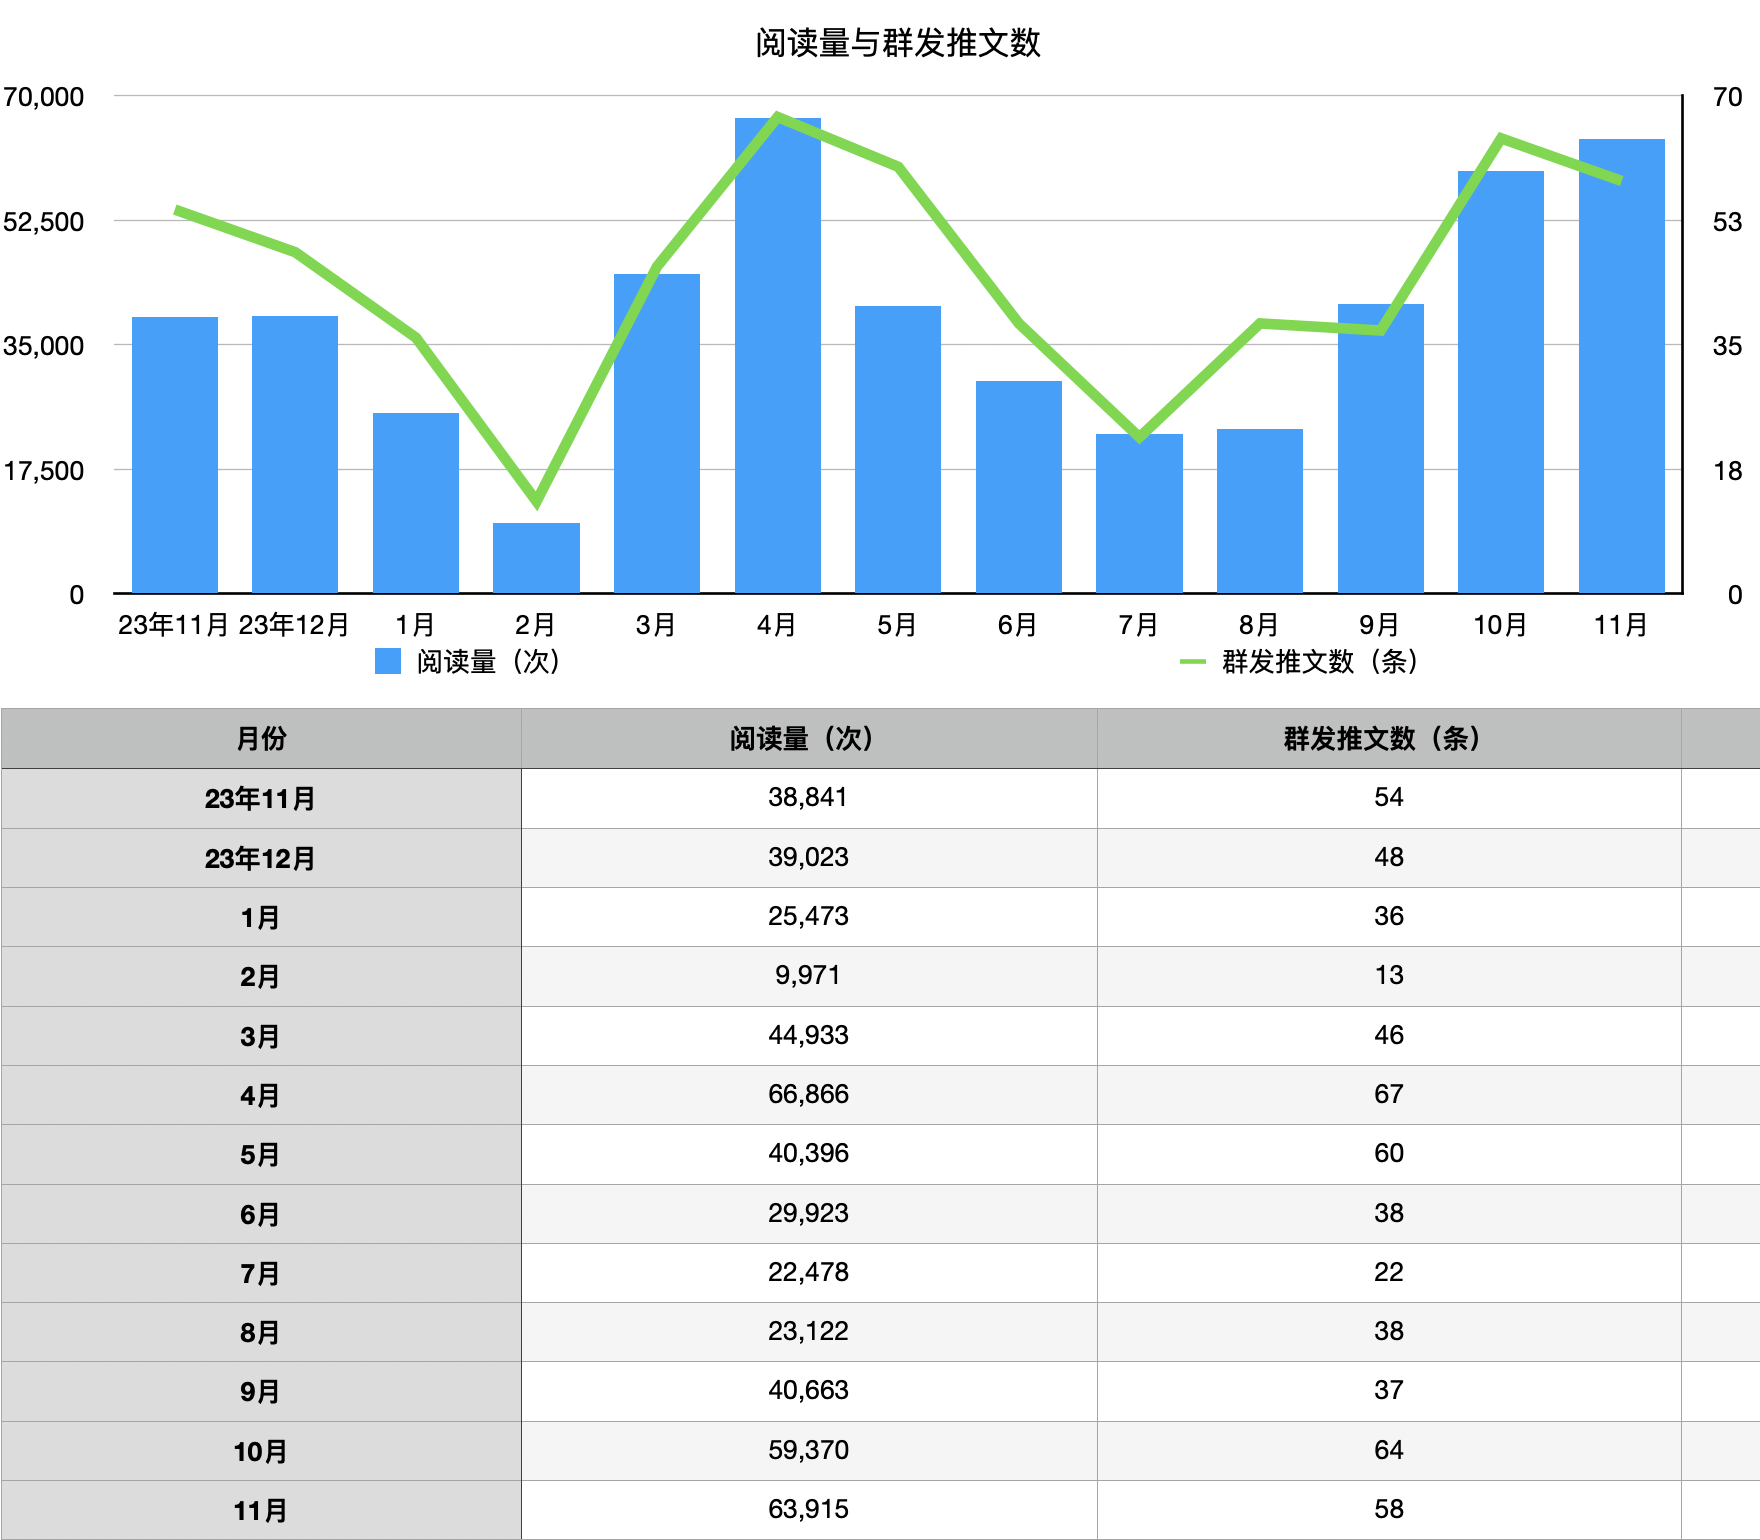
\includegraphics[width=0.8\textwidth]{Figure1.png} % 图片路径和宽度
    \caption{公众号阅读量与群发推文数} % 图片的标题
    \label{fig:example} % 图片的引用标签
\end{figure}

\subsection{活动拍摄}
新媒体中心在本年度承担了学院和学生会各部门各类活动的拍摄工作,为活动宣传工作的开展提供了有力支持。例如,文体部的红歌会、创赛中心的美赛宣讲会、学院迎新活动以及团学互访活动等重要活动,均由新媒体中心负责现场拍摄。本年度累计完成拍摄任务超过20次,通过高质量的照片记录了我院学生在各项活动中的风采,为学院活动留存了宝贵的影像资料。
\begin{figure} [H]
    \centering
    \includegraphics[width=0.8\textwidth]{Figure2.png} % 图片路径和宽度
    \caption{部门拍摄的部分活动} % 图片的标题
    \label{fig:example} % 图片的引用标签
\end{figure}
\subsection{海报制作}
新媒体中心在本年度积极承担了学院各类节气、节日以及重要活动的海报设计制作工作,共计完成海报30余张。这些设计紧扣主题,融入创意元素,涵盖了传统文化节气、校园节日庆祝以及学院重大活动等多方面内容。高质量的视觉宣传不仅营造了浓厚的校园文化氛围,也为活动的宣传工作提供了有力支持,并进一步彰显了学院的文化内涵和艺术魅力。
\begin{figure} [H]
    \centering
    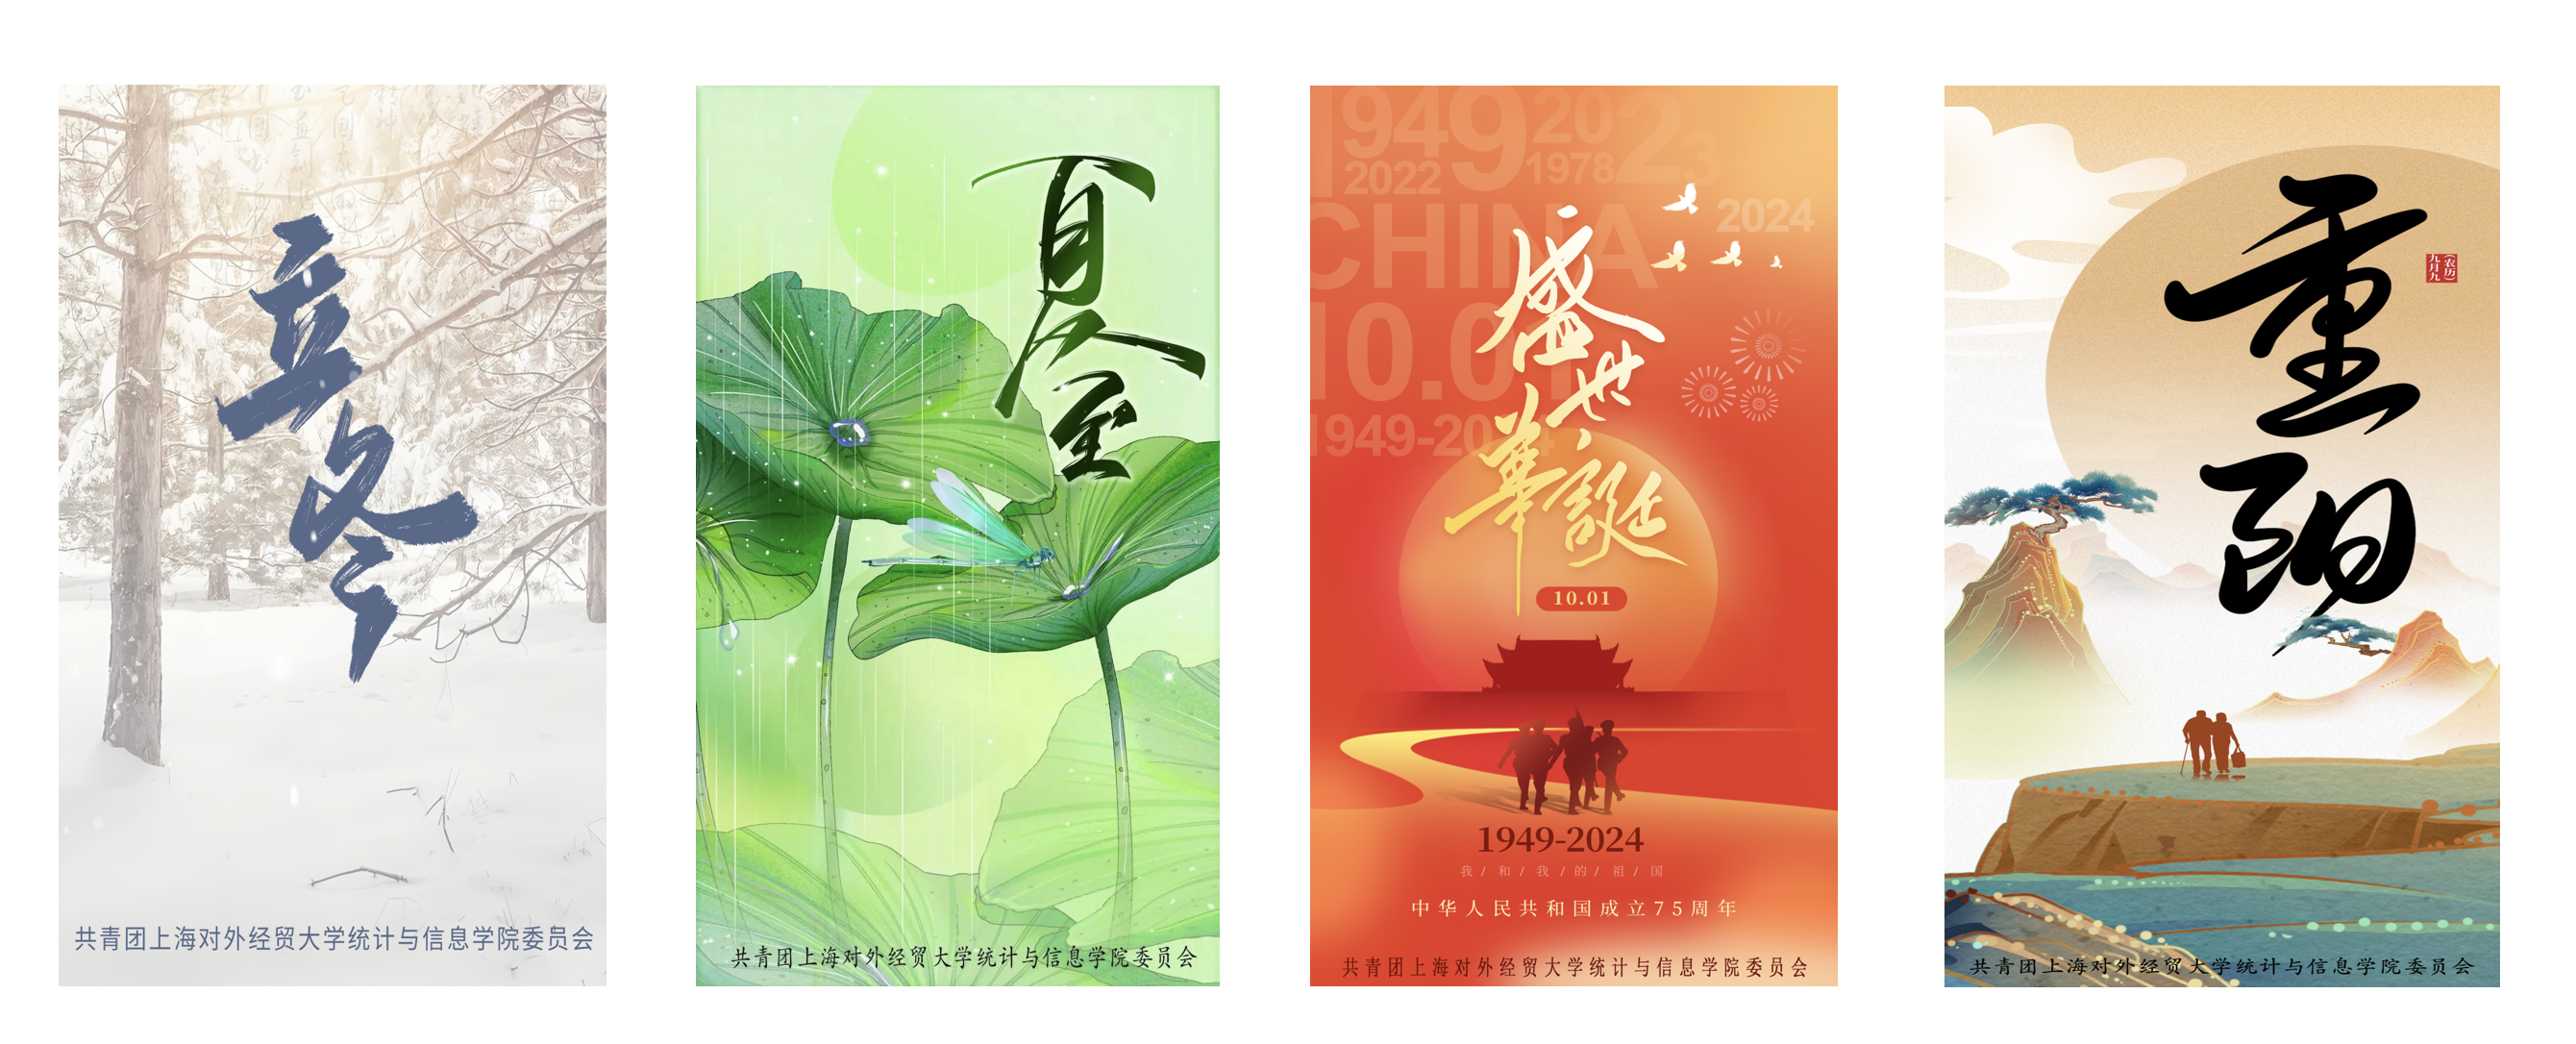
\includegraphics[width=0.8\textwidth]{Figure3.png} % 图片路径和宽度
    \caption{部门制作的部分海报} % 图片的标题
    \label{fig:example} % 图片的引用标签
\end{figure}
\subsection{活动承办}
本年度,新媒体中心成功策划并执行了多项具有影响力的线上与线下活动,如本部门于12月12日承办的“‘美’在于发现,发现他人之美主题活动”、以及于国庆期间举办的“迎国庆主题海报设计比赛”等。这些活动主题鲜明、形式多样,不仅丰富了校园文化生活,增强了学生的参与感与归属感,也通过新颖的活动形式进一步扩大了学院的影响力。
\begin{figure}[H]
    \centering
    % 第一张图片
    \begin{minipage}[b]{0.45\textwidth}
        \centering
        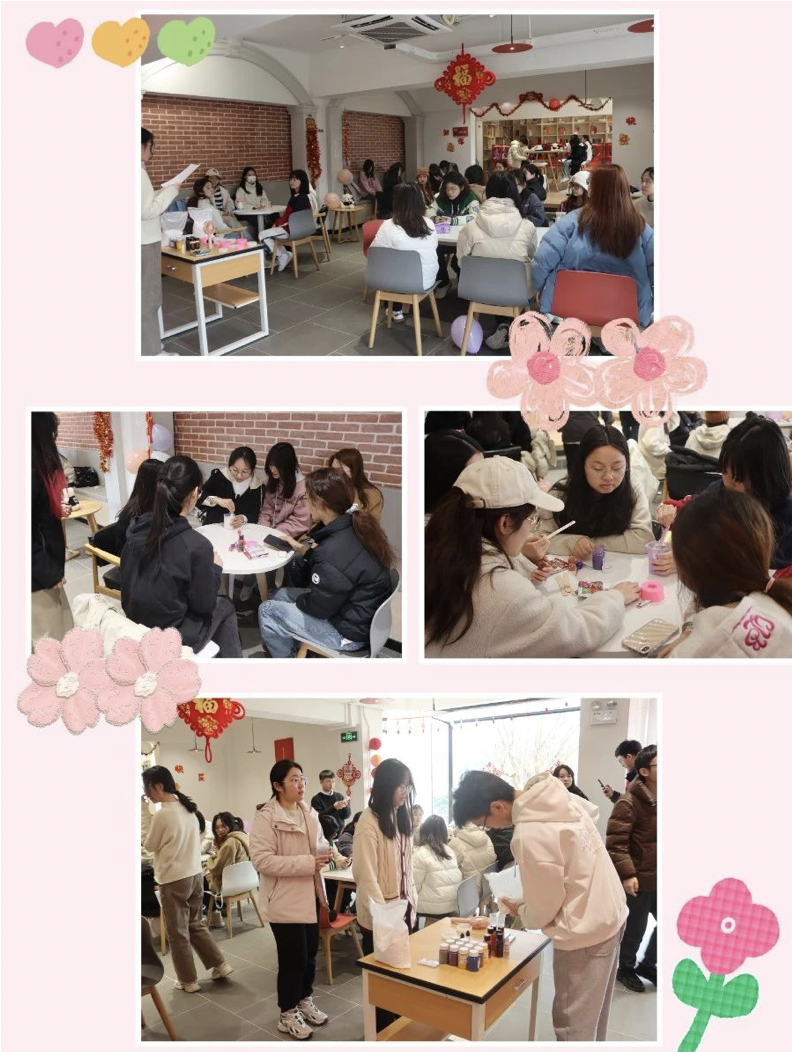
\includegraphics[width=\textwidth]{Figure4.png} % 替换为图片路径
        \caption{三八妇女节香薰石膏制作活动}
        \label{fig:image1}
    \end{minipage}
    % 第二张图片
    \begin{minipage}[b]{0.45\textwidth}
        \centering
        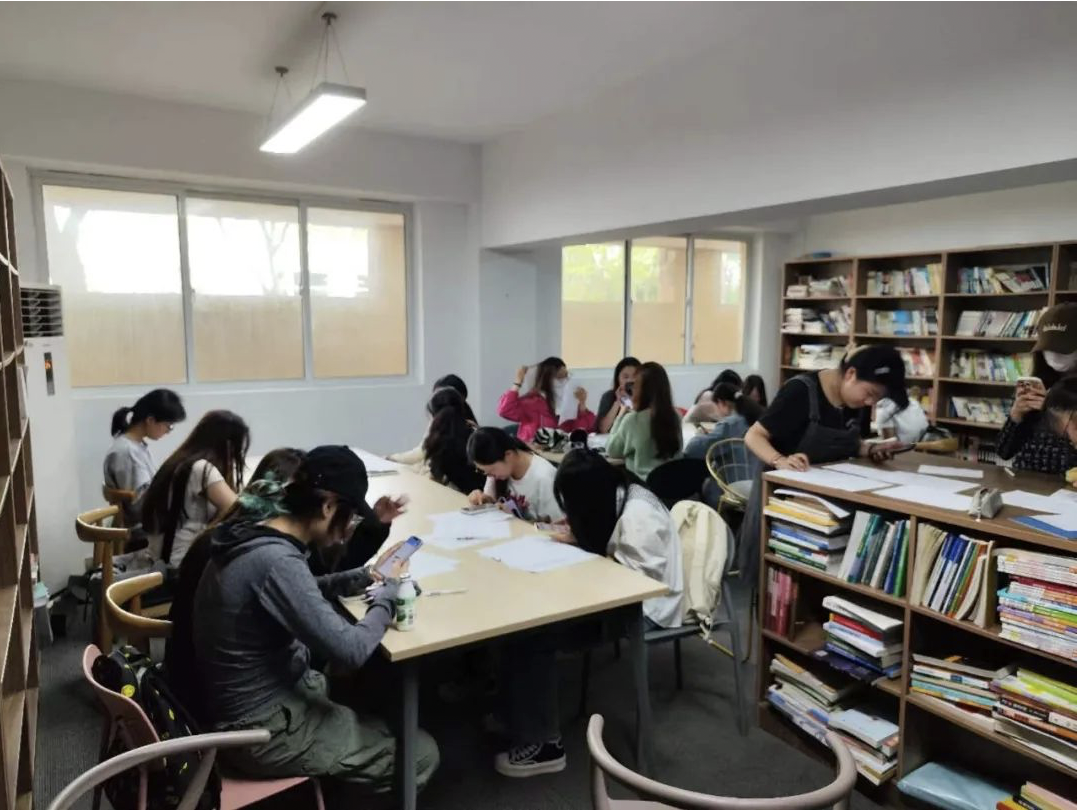
\includegraphics[width=\textwidth]{Figure5.png} % 替换为图片路径
        \caption{读书月拼贴诗活动}
        \label{fig:image2}
    \end{minipage}
\end{figure}

\section{工作亮点}
新媒体中心创新性地运用了AI绘图技术,将校园内的教学楼形象化为充满趣味的毛绒玩偶设计。这一创意既赋予了传统建筑全新的艺术表现形式,也能增强了学生对校园文化的认同感与亲近感。这展示了新媒体中心在内容创作上的创新能力和应用前沿技术的潜力。
\begin{figure}[H]
    \centering
    % 第一张图片
    \begin{minipage}[b]{0.45\textwidth}
        \centering
        \includegraphics[width=\textwidth]{J1.png} % 替换为图片路径
        \caption{原图}
        \label{fig:image1}
    \end{minipage}
    % 第二张图片
    \begin{minipage}[b]{0.45\textwidth}
        \centering
        
\includegraphics[width=\textwidth]{J2.png} % 替换为图片路径
        \caption{使用AI制作的图片}
        \label{fig:image2}
    \end{minipage}
\end{figure}
\section{部门团队建设}
本年度,新媒体中心吸纳了12名新成员,为新媒体中心注入了新鲜血液。新媒体中心高度重视新成员的培养与融入,针对技能提升进行了多次培训,包括推文编辑、海报设计、拍摄技巧等,帮助新成员快速掌握基础技能并适应工作节奏。我们也通过实际工作来对新成员进行技能培训,让他们实际参与推文编辑、海报设计、活动拍摄等任务,快速上手并积累经验。在每项工作中,部长们会为新成员提供指导与建议,帮助新成员不断改进,逐步掌握专业技能。这种实践学习的方式也增强了新成员对工作的理解和责任感,为他们更好地融入团队打下了基础。

\section{工作问题与反思}
\subsection{部门沟通问题}
由于新成员普遍性格较为内向,彼此之间都感到十分陌生,团队内部沟通存在一定障碍。未来新媒体中心将开展更多团队破冰活动和小组协作任务,鼓励成员之间加强交流和协作,建立良好的团队氛围。
\subsection{新成员能力有限}
尽管已经对新成员进行了技能培训,但他们仅仅掌握了一些基础操作,缺少对技能的深入理解。这不利于提升部门工作的效率,也会使得工作成果不够美观。未来我们会对成员进行更多指导,加深他们对技能的理解,让他们在实践中成长。
\subsection{创新性不强}
新媒体中心目前工作局限于活动拍摄、图片后期制作方面,工作的创新性不够,未能将当下流行的新型科技融合进工作中;公众号发表的推送同质化严重,在同学中的吸引力下降。接下来会尝试运用更多新兴技术来运营公众号、举办活动。
\section{未来展望}
未来,新媒体中心将以内容创新和技术升级为双引擎,推动部门工作实现新的突破。我们计划加强原创内容的开发,探索深度报道、专题访谈等多元化内容形式,进一步提升内容的深度和差异化,增强在学生群体中的吸引力。同时,将加大对新媒体技术的研究与应用,打造更加个性化和沉浸式的传播方式,为用户带来全新的体验感受。此外,我们将继续做好日常推送、拍摄与海报制作等基础工作,确保宣传任务的高效执行,为学院的文化传播和品牌建设保驾护航。同时,新媒体中心将加强与各部门的协作,确保信息发布的及时性和准确性,努力将公众号打造为覆盖面更广、影响力更强的学院资讯平台。
\section{结语}
本年度,新媒体中心在全体成员的共同努力下,圆满完成了各项工作任务,为学院宣传工作注入了新的活力与创意。从高效运营微信公众号、记录校园活动风采,到设计精美海报、成功策划特色活动,中心以务实的态度和创新的精神,展现了作为学院宣传窗口的核心价值。同时,我们也意识到,在团队沟通、成员能力提升以及工作创新性方面仍有许多改进空间。展望未来,新媒体中心将以更高的标准要求自己,在内容质量与技术应用上不断突破,进一步强化团队建设,优化工作流程,努力为学院文化传播和品牌形象建设贡献更大的力量!



\end{document}